\documentclass[12pt, a4papre]{article}
\usepackage[catalan]{babel}
\usepackage[unicode]{hyperref}
\usepackage{amsmath}
\usepackage{amssymb}
\usepackage{amsthm}
\usepackage{xifthen}
\usepackage{listings}
\usepackage{siunitx}
\usepackage{float}
\usepackage{graphicx}

\newcommand{\norm}[1]{\lvert #1 \rvert}
\graphicspath{ {./Images/} }

\hypersetup{
    colorlinks = true,
    linkcolor = blue
}

\author{Daniel Vilardell \\ Elias Ismael Estévez}
\title{Previ practica 1 ICOM}
\date{}

\begin{document}
	\maketitle
	\textbf{1.2:} Primer trobem el voltatge a un extrem del circuit obert
	
	\[
		V = \frac{50\si{\ohm}}{50\si{\ohm}}V_{i_{ef}} = \frac{200mV}{\sqrt{2}} = \frac{0.2}{\sqrt{2}} = 0.1\sqrt{2} V
	\]  
	
	A partir d'aquest podem trobar la potencia facilment.
	
	\[
		P = \frac{V^2}{R} = \frac{0.1\sqrt{2}}{50}^2 = \frac{0.02}{50} = 0.4 mW
	\]
	
	Finalment ho passem a dBm
	
	\[
		P|_{dBm} = 10log_10(0.4) = -4dBm
	\]
	
	\textbf{1.3:} 
	
	\begin{figure}[H]
		\begin{center}
		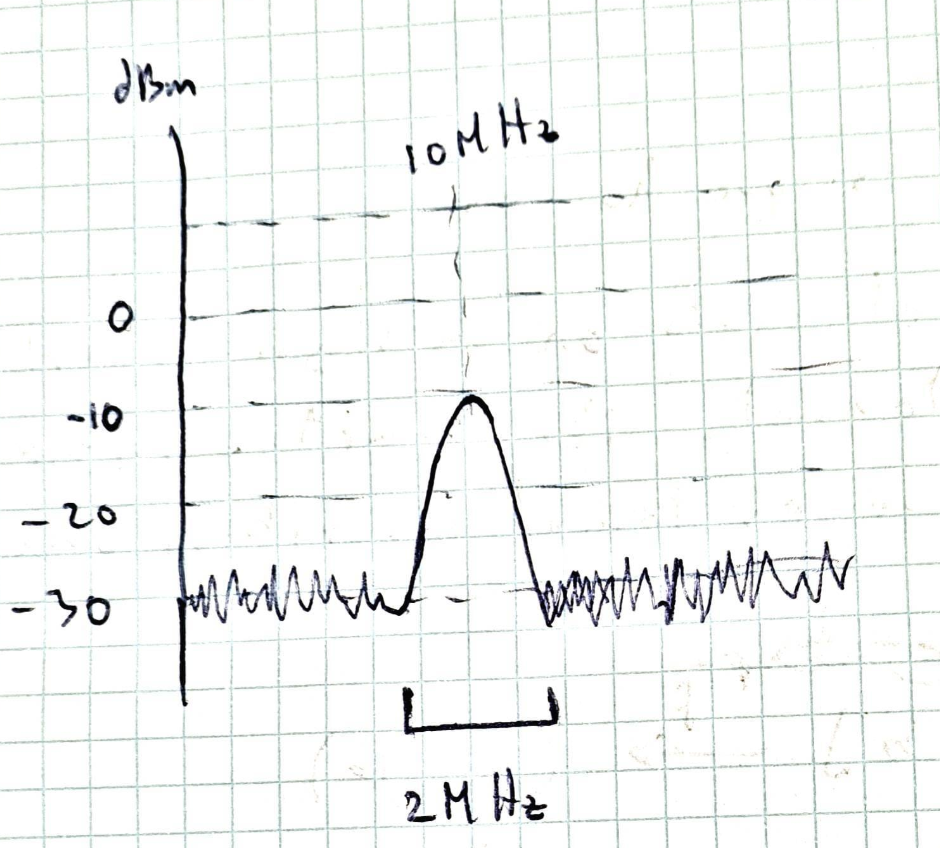
\includegraphics[width=70mm]{Previ_1.png}
		\caption{Dibuix de senyal vist per pantalla}
		\end{center}
	\end{figure}
	
	\textbf{1.4:} Per a que es veiessin les dos senyals igual de centrades hagafaria com a center frequency la mitjana entre les dos senyals, es a dir 
	
	\[
		f_c = \frac{10 + 25}{2} = 17.5MHz
	\]
	
	Com a RBW agafarem $RBW = 30kHz$ i per tal que es vegin be les dos senyals agafarem $Span = 25 - 10 + 2*RBW \approx 16MHz$.
	
	Es veuria de la següent manera:
	\begin{figure}[H]
		\begin{center}
		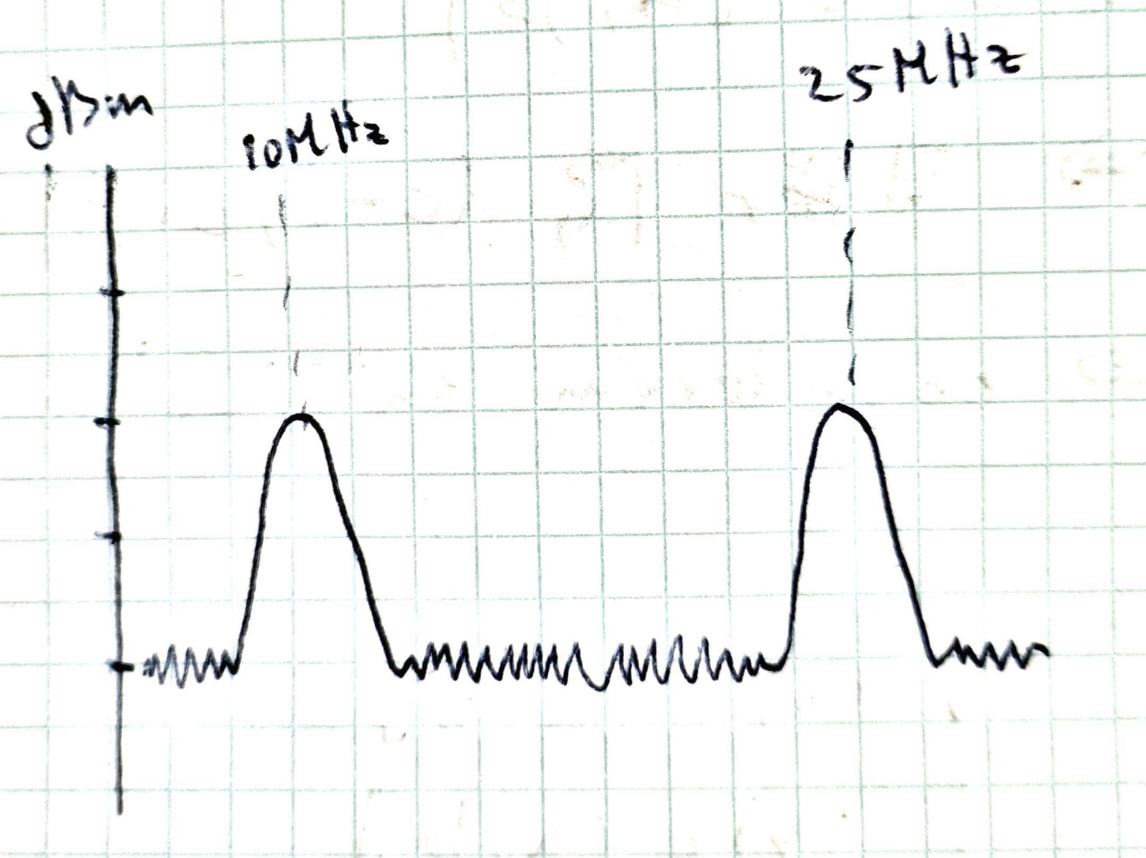
\includegraphics[width=110mm]{Previ_2.png}
		\caption{Dibuix de senyal vist per pantalla}
		\end{center}
	\end{figure}
	
	\textbf{1.5:} El nivell de pic del senyal s'atenuara i per tant serà inferior al original. El nivell de terra disminuira pero menys que el nivell de pic ja que s'atenua proporcionalment. Finalment l'amplada del lobul principal no es modificarà, ja que l'atenuació no afecta aquest parametre, sinó el RBW.
	
	
\end{document}










